\chapter{Dynamic 3D Object Insertion}\label{chp:ObjectLoading}

In order to realize the insertion of a 3D object from a CAD file, a plug-in with this functionality was developed simply called CADRuntimeImporter(CRI). Alongside it a standalone Unreal prototype project, named CADRuntimePresenter(CRP), was made that incorporates CRI in order to demonstrate how it can be used for a multi-user desktop and VR environment. The whole mechanism can be split into three major sections: opening and parsing the files, generating the objects and lastly user interaction with said objects. How all of that was implemented and what sort of advantages and disadvantages these approaches have, will be discussed in this chapter.
%%%%%%%%%%%%%%%%%%%%%%%%%%%%%%%%%%%%%%%%%%%%%%%%%%%%%%%%%%%%%%%%%%%%%%%%%%%%%%%%%%%%%%%%%%%%%%%%%%%%%%
\section{Loading and Parsing CAD Files}
\subsection{File Loading and Sharing}
The first step in creating an object in runtime is naturally opening the desired file and getting the required data from it in runtime. As Unreal Engine is written in C++, it is not surprising that opening up a file isn't too much of an issue. What makes this simpler is the fact that Unreal also offers this in their FileHelper class with the functions LoadFileToString() and LoadFileToArray(). The first function can load a text file into a string, while the other loads binary files into an array of bytes. This is only directly available in C++ and therefore had to be exposed to Blueprints. As this functionality is more of a utility, it isn't the best idea to attach it to a specific object. Luckily for such purposes Unreal offers Blueprint Function Libraries. This is just a special type of Unreal C++ class in which only static functions can be defined. These functions then become available to be used in any Blueprint without needing any instanced objects.\\

Something that is slightly more complicated is actually choosing the file. Here Unreal does technically offer the ability to open a file dialog but this is a strictly developer only module and can't be used in finished products. Even neglecting that, it wouldn't work in VR so a separate solution would have been needed anyway. Due to this a file picker in CRPs UI had to be written. The end result of that can be seen in Figure \ref{fig:FilePicker}. The design is rather simple but offers all the necessary functionality, especially that it is compatible with VR and only displays supported file formats.\\

\begin{figure}[htpb]
	\centering
	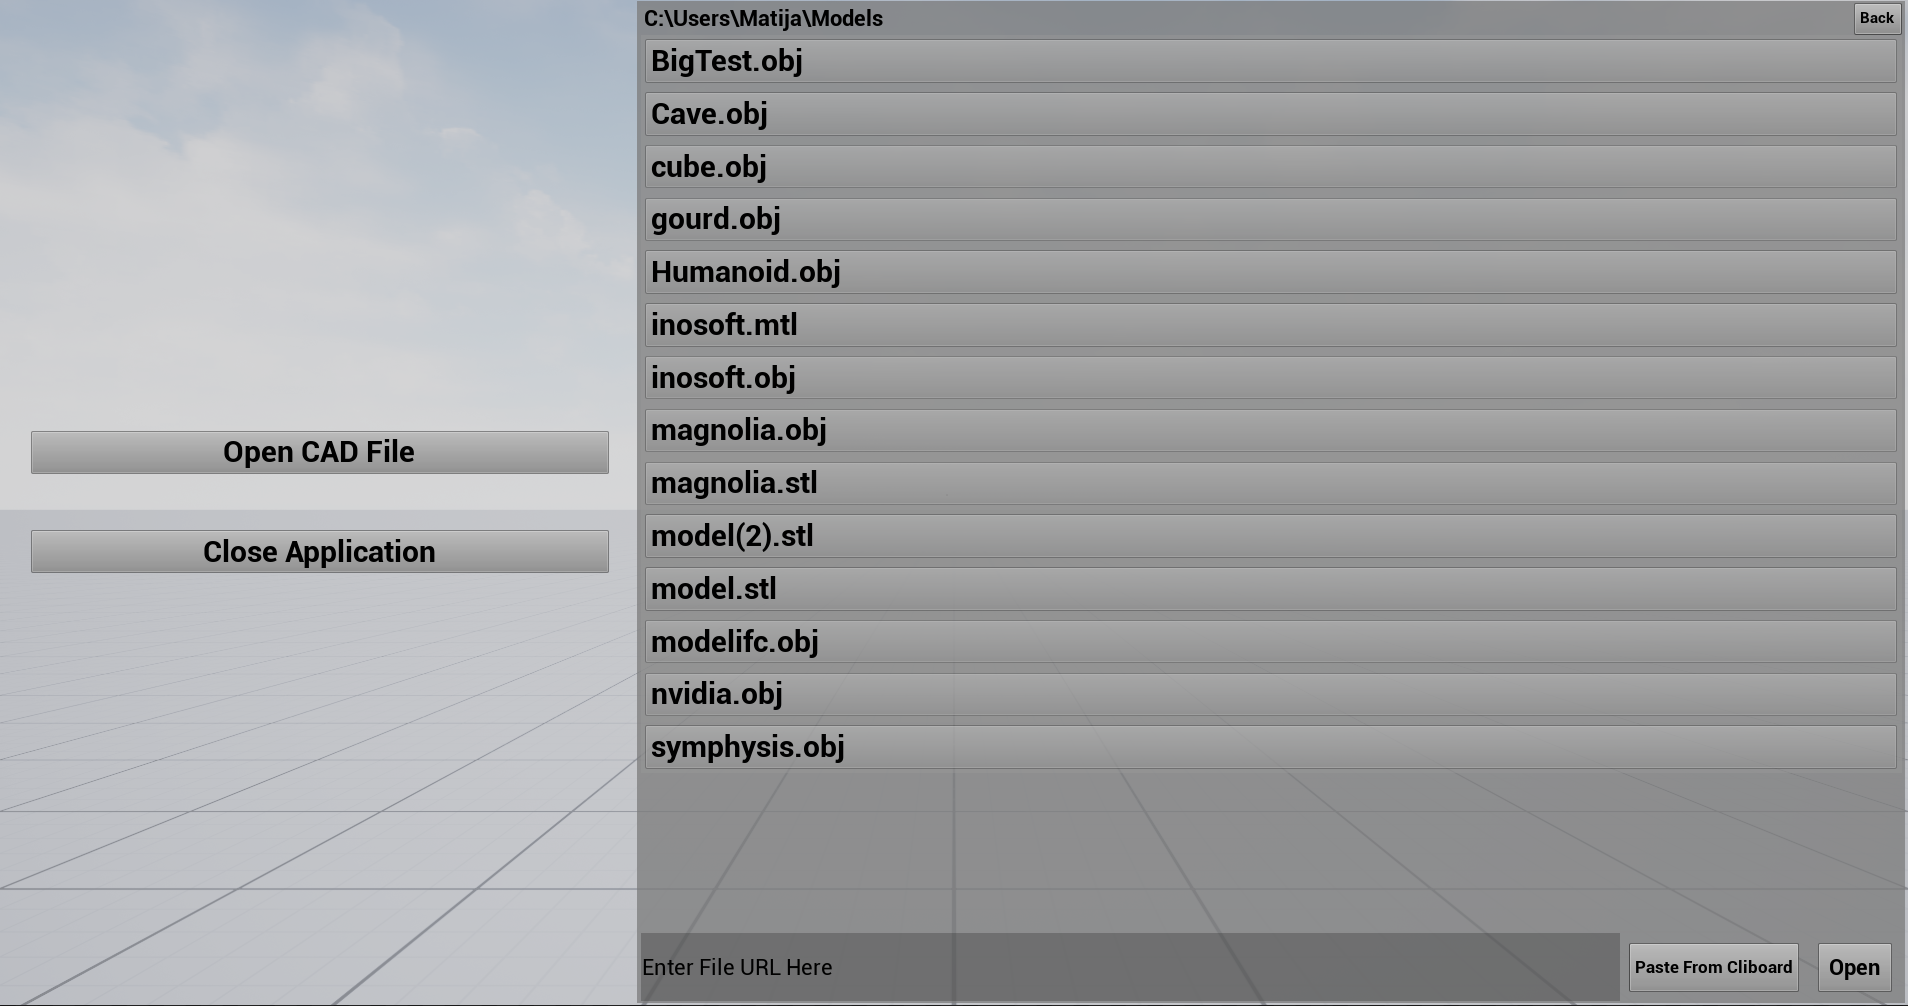
\includegraphics[width=0.9\textwidth]{fig/FilePicker2.png}
	\caption[CAD Runtime Presenter File Picker]{File Picker for CRP\protect}
	\label{fig:FilePicker}
\end{figure}

For a single user this would be enough, they could choose a file and then it could be parsed for object generation. Complications arise once there are multiple users involved. If a user were to open a file in such a scenario, the object would appear only in the world of that user and not for other users or even on the server. This could cause many issues since the clients world would not match servers, which is the authoritative instance. The problem lies in the fact that the new object needs to be created on every client and on the server. In order for that to happen every machine needs access to the required data, not just the client who has the file available on their machine.\\

One way of sharing this data is saving it in a replicated variable and having it handled by the automatic replication system. This does actually work but it has one fatal flaw which makes using it not viable. That is the size limit of replicated variables. The size limit for arrays is 64 kilobytes and for strings it seems to about the same. For smaller files this would be a perfect solution but unfortunately CAD files tend to be too big for it.\\
So instead this problem was solved by having the file be uploaded to a server and then be downloaded by the rest of the clients and server. For such purposes Unreal offers the HTTPModule interface, which uses the popular and powerful libcurl library, to create HTTP requests. A file could then be uploaded using a POST request and downloaded using a GET request. For this a simple file server which can handle such requests was written in python. The only problem is that the clients and server need to know where and what file was uploaded in order to make the correct request. This is where replication comes in handy. The client that uploads the file can tell the server where it was uploaded through a replicated string, which is most likely going to be within the size limit, and then the server can propagate that information to the rest of the clients which then make the GET requests.\\
Seeing as for most users only the link to the file matters, this means that the client that wants to open a file doesn't even need to have it locally on their machine. Instead they can simply input a link to a service like Dropbox or Google Drive and have everyone download those files. The UI for that is also part of the file picker and can be seen at the bottom of Figure \ref{fig:FilePicker}.\\
There are technically other libraries and plug-ins that could be used to enable file sharing with more complicated protocols but that wasn't necessary for this prototype project. The HTTPModule is simple to use while offering all the needed functionalities and avoids having to rely too much on third-party libraries.


%%%%%%%%%%%%%%%%%%%%%%%%%%%%%%%%%%%%%%%%%%%%%%%%%%%%%%%%%%%%%%%%%%%%%%%%%%%%%%%%%%%%%%%%%%%%%%%%%%%%%%
\subsection{Parsing Wavefront OBJ and STL}

Once every instance of the program has the desired file, the next step can begin which is parsing the data. What data is available and how it is stored can vary heavily from format to format. Generally they will all have the vertices that define the mesh but outside of that colour, material or anything else isn't guaranteed. This is the case because CAD formats tend to be highly specific for their uses cases, as well as proprietary for the CAD software they were developed for. This makes supporting many CAD formats quite difficult, especially those that aren't well documented or don't even have publicly available documentation. Considering the scope of this project, spending too much time writing parsers for as many formats as possible was not feasible.\\
Instead the decision was made to use well known and widely supported formats, like OBJ and STL. One of the biggest benefits of this approach is the already existing support that these formats have. Many CAD softwares support exporting to one of these and even if they don't, there are probably tools with which the files can be converted. This saved a lot of time in the development, as only a few parsers had to be written and for those that had to be implemented, the process was fairly simple due to all the existing resources on the formats.

\subsubsection{Wavefront OBJ}

Wavefront OBJ, or simply OBJ, is a geometry definition file format developed by Wavefront Technologies for their Advanced Visualizer animation packages. It is a neutral, open source format which has been widely adopted and has good import and export support from almost all CAD software.\\
Another reason why OBJ was chosen is the fact that is can be directly read through any text editor. This helped out a lot in early stages of development where the primary goal was to prove that the concept worked. Being able to see and read the data made it simpler to write a parser in the first place, as well as comprehending what was going on with the data at later stages.\\ 
The format represents 3D geometry in the form of vertex positions, vertex normals, texture coordinates, polygonal faces and groups of faces. These geometries can also use materials indirectly through referencing materials defined in a separate MTL file. Every entry in an OBJ file is represented through a single line, starting with an identifying tag followed by the value of the entry. What these entries can look like is represented in Table \ref{tab:ObjTypes}.

\begin{table}[htbp]
	\centering 
	\scalebox{0.889}{
		\begin{tabular}{lll}
			\toprule \textbf{Tag} & \textbf{Example Value} & \textbf{Definition} \\
			\bottomrule
			v & 0.2 0.3 0.5 & 3D Vector representing 3D Vertex \\
			vn & 1.0 0.5 0.0 & 3D Vector representing 3D Normal \\
			vt & 0.5 0.25 & 2D Vector representing Texture Coordinate\\
			f & 1/1/2  2/2/5  3/3/5 & Polygonal Face made from Vertices, Normals and Textures\\
			usemtl & Stone & Defines what Material should be used for following faces\\
			g & Door & Defines a polygon group\\
			\bottomrule
	\end{tabular}}
	\caption[ObjTypes]{Relevant types in OBJ format}
	\label{tab:ObjTypes}
\end{table}

In order to parse their values, most of the entries can be regarded one-by-one. Vertices, normals and texture coordinates are vectors and can be saved in separate vector arrays in the order in which they appear. How these and the rest of the values are used will be explained later, for now it's only important how they are saved.\\
Faces, materials and group are more complicated as they define how the rest of the data is put together to make the object. A face represents a polygon defined through lists of vertex, texture and normal indices in the format "vertexIndex/textureIndex/normalIndex", as can be seen in Table \ref{tab:ObjTypes}. It is important to note that these are the indices of the values and not the values themselves. Also the indices for vertices, texture coordinates and normals are separate and based on when the entry was defined in the file starting with one. So both a vector and normal can have their respective index be 1. The polygons themselves tend to be triangles but can also have more sides. This isn't ideal as later for generating the mesh, only triangles are supported but there is a simple way to solve this. The vertices are listed in a counter clockwise order so that any polygon can be represented through a triangle fan, as is shown in Figure \ref{fig:TriangleFan}. So faces that define polygons with more than 3 edges are replaced through multiple triangular faces.

\begin{figure}[htpb]
	\centering
	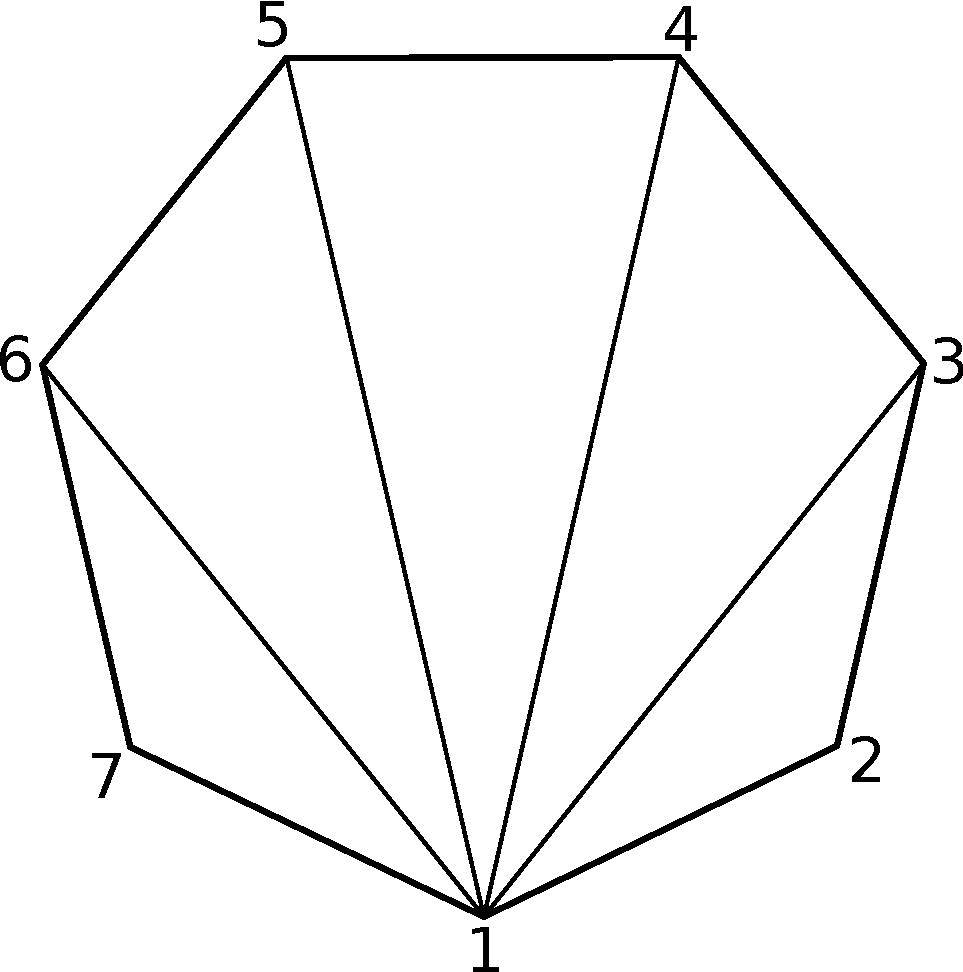
\includegraphics[width=0.3\textwidth]{fig/TriangleFan.pdf}
	\caption[OBJ Polygon to Triangle Fan]{Polygon represented through a Triangle Fan\protect}
	\label{fig:TriangleFan}
\end{figure}

A group determines what faces are combined in order to make a component of the larger object. The "usemtl" tags tells what material should be used on the faces and that material is used until the next tag appears. The actual materials are defined in an MTL file, which works similarly to an OBJ, just with different tags and values. Some of the more important entries can be seen in Table \ref{tab:MTLTypes}. This MTL file of course also needs to be shared to every client. The values themselves are saved in a Map where the keys are the material names and the values are arrays of the values.

\begin{table}[htbp]
	\centering 
	\scalebox{0.889}{
		\begin{tabular}{lll}
			\toprule \textbf{Tag} & \textbf{Example Value} & \textbf{Definition} \\
			\bottomrule
			newmtl & Stone & Defines the name of a new Material\\
			Ka & 1.0 1.0 1.0 & Ambient colour\\
			Kd & 0.0 0.0 0.0 &  Diffuse Colour\\
			Ns & 1.0 & Specular Exponent\\
			d & 0.5 & Transparency\\
			
			\bottomrule
	\end{tabular}}
	\caption[MTL Types]{Relevant types in MTL format}
	\label{tab:MTLTypes}
\end{table}

As the information of these values heavily relies on each other, they needed to be combined and saved in an array where every array entry represents one component of the whole object. The entry consists of the face values and marks where materials need to be switched.\\
The only major problem with OBJ is the fact that the coordinates don't have units, meaning they can't be scaled to properly represent the designed size. Instead everything is scaled with same factor so that at least the scales between objects made in the same scene stay the same. Also the created objects can later be scaled by users to better resemble the desired size.

\subsubsection{STL}
STL is a file format native to the CAD software created by 3D Systems in 1987\cite{}. The format has gained a lot of support in many different software packages, especially for 3D printing software where it is one of the default formats. STL files only describe the surface geometry of a three-dimensional object with out any additional information about colours, materials or groups. The geometry is described in raw, unstructured triangles defined by a normal and three vertices. The way a triangle is defined in the file is shown in Figure \ref{fig:STLFormat}. 
\begin{figure}[htpb]
	\centering
	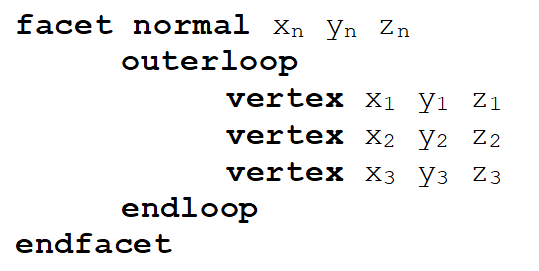
\includegraphics[width=0.35\textwidth]{fig/STLFormat.png}
	\caption[STL Triangle facet]{A triangle facet represented in STL\protect}
	\label{fig:STLFormat}
\end{figure}

While the structure suggests that multiple possibilities are possible for loops, the facets can only be triangles. In order to represent a full model the triangles are simply listed one after the other. In order to parse it, the vertices and normals are saved in arrays and faces are generated to point what vertices make up the triangles. This is important for generating the mesh later. While it is a simpler format compared to OBJ, it is excellent when only the shape is relevant. It does unfortunately suffer from the same scaling problems as OBJ and that is handled in the same way as well.\\
Overall with these two formats the majority of the most common and well-known CAD formats are covered. Ideally more formats would be covered and specific parsers for every format would be written to get the most accurate results but for the limitations of this project, this is a very practical solution.

%%%%%%%%%%%%%%%%%%%%%%%%%%%%%%%%%%%%%%%%%%%%%%%%%%%%%%%%%%%%%%%%%%%%%%%%%%%%%%%%%%%%%%%%%%%%%%%%%%%%%%%%%%%%%%
\section{Runtime Mesh Generation}

After the files have been parsed and the needed data was extracted, the actual process of creating a new 3D object starts. For that, a way to tell Unreal to generate a mesh is required and Unreal does in fact support such a feature in the form of so called Procedural Mesh Components(PMC). These components can be created in runtime by giving them the required mesh data and letting them generate themselves. In the first phases of this project it was explored as to how viable using these components were, seeing as they initially seemed to be exactly what was needed. Getting it to function took a bit of work, mostly due to Unreal Engines generally bad documentation, but the first results with small objects were quite promising. Unfortunately the problems started to arise with larger objects where the performance would drop significantly or the Unreal editor would simply crash. The reason for this lies within the procedural mesh components themselves. As the name implies, these components are supposed to be generated by some form of procedure which generally won't create nearly as many vertices as a large CAD file can. On top of that the underlying architecture for a real procedural system for expensive geometrical operations would be quite different to that of a runtime gameplay framework \cite{}. PMC is also a relatively late addition to Unreal Engine, first appearing in version 4.8 in 2015. So even though it is designed for a quite similar purpose, it is different enough that it couldn't be used.\\

Due to this a different method of getting Unreal to generate meshes had to be found and during this time a the most important question for this project came up. Doesn't Unreal technically already support runtime mesh generation? Let's say, as an example, there was an Actor that had some sort of static mesh attached to it. Unreal could spawn in this new Actor without a problem. So shouldn't it be able to create such an Actor from data parsed from a file?\\
A definitive answer for that question couldn't be found but through some research a few speculations can be made. The biggest reason for this probably stems from the main purpose of Unreal Engine. Unreal has always and will probably always be a video game engine. As such it is designed and optimized for use cases that happen in video games. In a game, every asset and model is carefully crafted and placed in a level. These objects are already known to the game and are packaged within it in an optimized state. The game knows exactly what to do with these and where to load them. That is a part of the core functionality of Unreal. But it isn't exposed directly to a developer because adding externals models to a game isn't generally required. Why should a game depend on the user having some specific type of file to load? Those need to be within the game itself. Not to mention the problems and security issues an external file could cause.\\
Another factor that comes into play are the hardware limitations that existed throughout most of Unreal's lifespan. Computers and gaming consoles weren't always as powerful as they are now, especially consoles tend to be very underpowered machines. As such a lot of work went into optimizing games so that they would run smoothly on their target platforms. Even nowadays with modern systems that are way faster, optimizing is a big part of game development. Especially important for that is managing what is loaded in and when as the systems can have limited memory. Some games will use a loading screen to hide the loading, other games might use a gameplay sequence that slows down the player so the game has time to load in the next assets. There are even games that would restart the console they were running on without letting the player know when the memory was full\cite{}. How these assets were stored also played a big role. Some games would use the same asset but with different colours to save space or some games saved the same asset multiple times so it could be accessed from storage quicker\cite{}. CAD files on the other hand tend to be rather big and just creating the files is already a very demanding job which requires good hardware. Due to all of this, the idea of just creating a new external model using Unreal's functionality isn't of value to game development and isn't directly exposed.\\
However Unreal isn't just a game engine any more. As already mentioned it has gained popularity in various fields and those have very different demands compared to games. This has led to many new additions to Unreal, most importantly Datasmith. Datasmith is a set of tools and plug-ins developed by Epic Games with the goal of streamlining the process of importing CAD files into the engine during development. It is a relatively new addition to Unreal as it was first released around 2016. CAD objects are very different to objects used in game development, they focus on creating geometry for manufacturing and production while game objects are more focused on looking a certain way and being optimized. Due to this, it is clear that this addition isn't meant for game development. But it wasn't until August of 2021 with the release of Unreal Engine version 4.27 and with it the release of the Datasmith Runtime plug-in that it gained the ability to import meshes in runtime. This plug-in, as it is still very new, is in beta and still being worked on. Most importantly it shows that with access to the mesh generation functionality of Unreal it is possible to create meshes from external data in runtime.\\ 

But the demand for such a functionality has existed for a lot longer and Unreal's existing solution with PMC wasn't good enough, which led to the development of Runtime Mesh Component (RMC). RMC is a third-party plug-in developed that exposes the mesh generation capabilities of Unreal in a much more efficient and feature-rich way compared to PMC. It promises 50-90 \% lower memory usage and 30-100 \% lower render thread CPU time \cite{} compared to PMC. These claims were checked and the results do match the expected improvements. It is also completely free and has been used in many projects even in larger companies \cite{}. This is why it was finally decided to use RMC for the purposes of this project. While ideally this project wouldn't need to rely on an unofficial plug-in, trying to recreate what is available with RMC, which has been around for more than 6 years and had more than 40 people contribute it, is not a feasible endeavour. Instead, for the limitations of this project, it is much wiser to use this tool and apply its  capabilities for the purposes of generating CAD models.

\subsubsection{Generating a CAD Model}

% setiing up the class
%generating componenet individually through function sections
%attaching it and making it part of the actor
%setting it's relative position and setting the components 
%sections differ based on material as only one material per section is allowed
% creating the materials
Before a model can be generated, there needs to be an Actor to which the components can be attached to. Technically this could be any Actor, even the Player Character, but it makes more sense to create a specific Actor for these purposes. In the plug-in such an Actor is defined in the CRIObject Blueprint class. Actors of this class are also going to be where the values from the parsed files will be stored, as well as the Actors that call the function to generate the new components on themselves.\\
In order to spawn in a new Actor of this class, the Unreal SpawnActor function can be used. This function just needs to know what class should be spawned and where. The first parameter is easy but the second one has a few more options. Depending on what is needed all these Actors could be spawned in the same place or a user could enter the coordinates. For the purposes of CRP it was decided that the location of the new Actor is going to be where the user adding the object is looking. For this the users camera rotation is taken as a forward vector, multiplied by a distance and added to the players location. The distance is based on the size of the spawned object so that collision is avoided but it also isn't spawned to far from the user. Also this spawning process happens as soon as clients start downloading the CAD files so that once the files are parsed, there is a place to save the data. The Actors will be in the world but won't be visible or interactive as they don't have any components yet.\\
Once the data has been saved, flags in the Actor get set in order to notify it that generating can begin. This is done because there is no guarantee that the CAD and material file will be downloaded in any specific order and generating before all the needed data is there would cause problems. The material flag is also only used if the file uses it and the user specified that it should be created with materials.\\
The whole model isn't generated all at once because this could cause the program to stutter or freeze for the duration of the process for larger files. This happens due to this running on the same thread as the main thread, which means that nothing is rendered until this is finished. Instead each component gets generated separately from the rest in the order that they are defined in the file. This is realized through the tick event that Actors can possess. A tick event is simply an event that gets called every frame or in some other interval. As the components themselves are comparatively small, generating one doesn't cause a significant performance hit that could freeze the main thread. So basically by doing this, the performance cost of generating the model gets spread across every component and becomes practically negligible. Another benefit of this is the fact that the components themself start appearing one after the other in the world, creating an interesting-looking animation. Ideally multithreading would be used for even better results but Unreal is rather specific about that due to its built-in garbage collection\cite{}.\\
With every tick the GenerateMeshComponent function is called and a counter is kept as to know what components have already been dealt with. The function is implemented in C++ as the performance is necessary but in order to call it from Blueprints it was implemented in a Blueprint Function library, just like the file reading function. It could also have been implemented as a native function of the CRIObject class but, as this is supposed to function as a plug-in, it didn't make sense to limit it to one specific class. This way the functionality can be used in more ways depending on what the user needs. One such way is implemented in CRP and will be demonstrated later.\\
How the function works can be seen in Algorithm \ref{algo:MeshGeneration} which shows the process in a simplified pseudocode.

\begin{algorithm}[htpb]
	\texttt{Input} $Actor, ComponentIndex, Vertices, TextCoords, Normals, \linebreak \null \quad\quad \quad ComponentData, Materials, UseCollision;$\\
	$RMC = new \: CustomRuntimeMeshComponent()$\\
	$RMC.ID = ComponentIndex$\\
	$RMC.AttachTo(Actor)$\\
	$RMC.UseCollision = UseCollision$\\
	$Center = FindBoundingBoxMiddle()$\\
	$RMC.SetRelativeLocation(Center)$\\
	$Vertices.Translate(-Center)$\\
	$RMC.CenterVertex = Center$\\
	$Secitons = GetComponentSections(ComponentData)$\\
	$SectionMaterials = GetSectionMaterials(Materials)$\\
	\texttt{for} $i := 0$ \texttt{to} $Sections.Length$ ~\texttt{do}\\
	\hspace{5mm} $Faces = GetFacesForSection(Sections[i])$\\
	\hspace{5mm} $Material = SetupSectionMaterial(ComponentMaterials[i])$\\
	\hspace{5mm} $RMC.CreateSection(i, Vertices, Faces, Normals, TexCoords, Material)\newline$\\
	
	\caption{Pseudocode for generating a Mesh Component}
	\label{algo:MeshGeneration}
\end{algorithm}

As can be seen the function takes quite a few inputs but all of those necessary. The first step is instancing a new Runtime Mesh Component object. In this case it is a slightly customized subclass of RMC that contains a few more variables that can be quite useful. One of those being the index of component, which is used when interacting with components. After that the component is attached to the Actor generating it as it cannot exist in a scene on its own. Based on user wishes the mesh can be created either with or without collision. Next the a bounding box is generated from the vertices of the component and the centre of that box is determined. This is done because when a component is added to an Actor, its relative location is (0,0,0) so it's in the centre of the Actor. The mesh on other hand will be placed where the vertices are. Once the whole mesh is generated it will look exactly the way it should but there will be problems with certain interaction. Let's take rotation as an example. Since the position of the component is technically in the centre of the object, rotating it will cause the mesh to rotate around the whole object instead of itself. In order to fix that, the component is placed where the centre of the mesh will be and the vertices are translated the same amount just in the opposite direction. These two translations cancel each other out so that the whole mesh ends up looking unchanged. Meanwhile the position of the component matches the centre of the mesh so that rotating and scaling work properly. Alternatively the component could be moved and translated in specific ways to simulate such a rotation but this is many times more complicated and unnecessary. The location of the centre is also saved in the custom class as it is required for some interactions that will be explained later.\\
Then the component is split into sections and the material values for the sections are extracted. An RMC can contain one or multiple meshes and these are regraded as sections. In this case the mesh is split according to the materials seeing as a section can only use one material. This way a component can have multiple meshes, instead of having to create a component for every material change. Lastly for every section, all the indices defining its faces are saved in one array and the appropriate material for it is setup. In Unreal a completely new material cannot be created at runtime. Instead an already existing material is needed as the parent for an instance of a dynamic material. Such a dynamic material can be create during gameplay and the values that define it can be altered as well. There is just a slight problem du to the plug-ins current limitations. The materials in Unreal are physically based rendering(PBR) materials, while the MTL uses Phong shaded materials. These two ways of rendering are vastly different and there isn't one true way of converting between them. That's why the diffuse colour, specular exponent and opacity are used to approximate the appropriate values for the PBR material. How well this works depends on what material is supposed to be represented. This is slightly unfortunate but what is more important is the fact that an appropriate material could technically be created. If a new format, that supports PBR, were to be added the whole mesh generating approach would still be the same just with the correct values. Also technically two parent material are needed, one for opaque and one for translucent materials because of the way Unreal handles opacity.\\
Finally the RMC takes all of the inputs that it needs and creates a section. This is then repeated for every section of every component until the whole mesh has finished generating. The model will appear in the world in the position where the Actor was spawned and the result of such a process can be seen in Figure \ref{fig:LoadedModel}.

\begin{figure}[htpb]
	\centering
	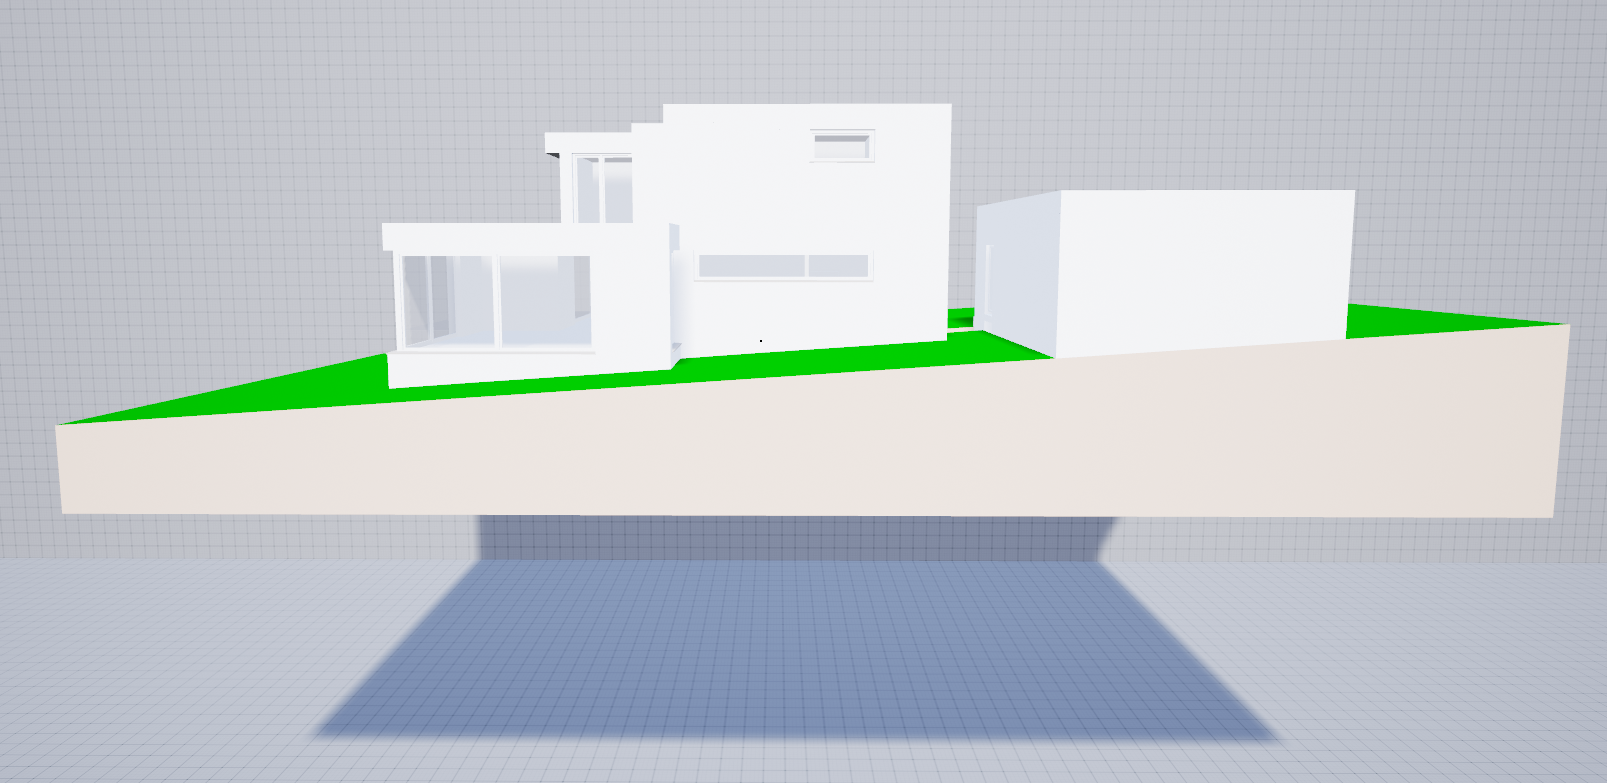
\includegraphics[width=0.675\textwidth]{fig/LoadedModel2.png}
	\caption[Loaded CAD Model in Unreal Engine]{Loaded CAD Model in Unreal Engine\protect}
	\label{fig:LoadedModel}
\end{figure}

%%%%%%%%%%%%%%%%%%%%%%%%%%%%%%%%%%%%%%%%%%%%%%%%%%%%%%%%%%%%%%%%%%%%%%%%%%%%%%%%%%%%%%%%%%%%%%%%%%%%%%%%%%%%%%

\section{Object Interaction}\label{chp:ObjectInteraction}
While being able to generate 3D models on its own is very useful, it would be severely limited if it just stood in a place and the users had no way of doing anything with it. That is why it is important to take a look at how it possible to interact with these objects. There are many ways in which this can be done so the presented solutions are just what was implemented in CRP to demonstrate some of the more essential interactions that can probably find use in most projects.
Most of the interaction was written in the Player Controller, while movement and looking around is handled in the Pawns. This was done because the Pawns have to be different in desktop and VR mode and that would mean writing pretty much the same code in two. Instead by having one Controller class and checking what mode is used, makes for much cleaner code and a more unified experience between the two modes.
\subsection{Grabbing and Translating}

One of the most basic but also important interactions a user can have with an object is grabbing and moving it around in the world. This is triggered when the user presses the grab button and stays as long as that button is held. Depending on the mode, this button is either the left mouse button or a trigger on a VR controller. When the button is pressed an RPC is called onto the server, where all of the interactions happen, that checks if the user is currently pointing at an object. 

\begin{figure}[htpb]
	\centering
	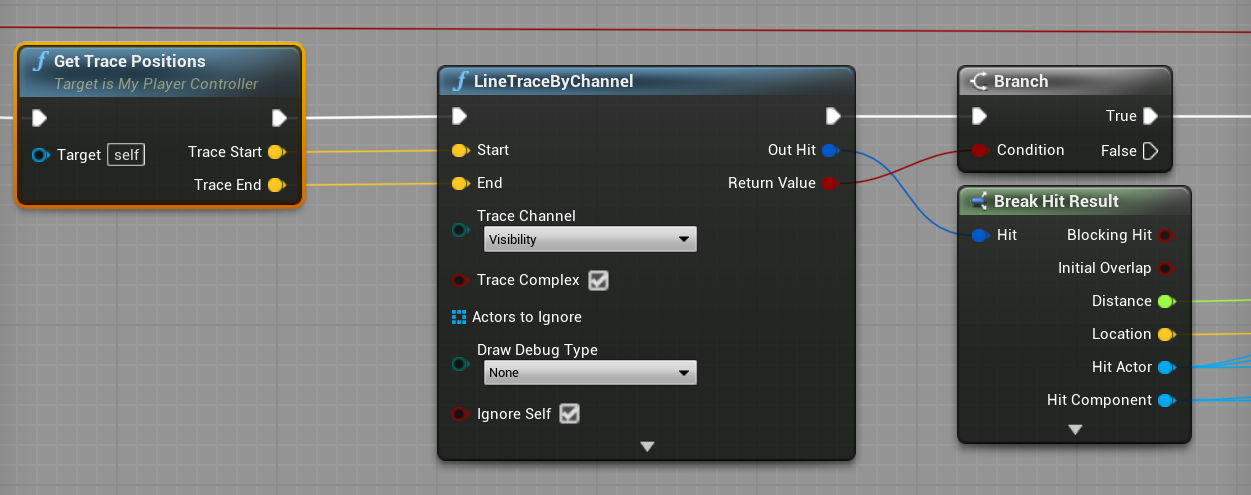
\includegraphics[width=0.8\textwidth]{fig/LineTracing.png}
	\caption[Tracing Grabs in Blueprints]{Tracing Grabs in Blueprints\protect}
	\label{fig:LineTracing}
\end{figure}
\subsection{Grabbing Individual Components}

As already mentioned, the model generally consists of many smaller components and while it is great to be able to interact with it as a whole, it could be a lot more useful if a user could choose to interact with every component individually.
%hovering

\subsection{Scaling and Rotating}

\subsection{Duplication, Expansion and Deletion}



